% beautiful title slides in Beamer
% Model 2
% latex-beamer.com

\documentclass[aspectratio=169, compress]{beamer}

\usetheme[
    outer/progressbar=foot, 
    sectionpage=progressbar,
    subsectionpage=progressbar, 
    numbering=counter
]{metropolis}
\setbeamertemplate{subsection page}[numbered]
\setbeamertemplate{subsection in toc}[subsections numbered]
%\setbeamertemplate{frame footer}{\insertsectionhead}
%\setbeamertemplate{progress bar in head}{\insertsectionhead}
\usepackage{natbib}
\usepackage{bibentry}

\setbeamertemplate{navigation symbols}{}
\setbeamertemplate{caption}[numbered]

\useoutertheme[subsection=false]{miniframes} %<<<<<<<<<<<<<<<<
\setbeamercolor{section in head/foot}{fg=white, bg=mDarkTeal} %<<<<<<<<<<<<<<<<
%\setbeamercolor{subsection in head/foot}{fg=white, bg=mDarkTeal} %<<<<<<<
%\setbeamercolor{title in head/foot}{fg=black, bg=white!50!MSUgreen} %<<<<<<<<<<<<<<<<


\usepackage{appendixnumberbeamer}
\usepackage{booktabs}
\usepackage[scale=2]{ccicons}


\title{Refrigeración en centros de procesamiento de datos}
\date{\today}
\author{Ana Buendía Ruiz-Azuaga \and Andrés Millán Muñoz \and Paula Villanueva Núñez} 
\institute{Universidad de Granada}

\begin{document}
\maketitle

\begin{frame}{Tabla de contenidos}
    \setbeamertemplate{section in toc}[sections numbered]
    \tableofcontents
\end{frame}




\section{Introducción}    

\begin{frame}{Introducción}
    \begin{enumerate}
        \item \textbf{Centros de procesamiento de datos} en auge por la computación en la nube.
        \item Aumenta la densidad de componentes por unidad de espacio.
        \item \textbf{Sistemas de refrigeración} esenciales para disipar el calor generado. 
    \end{enumerate}    
\end{frame}




\section{Preliminares}

\begin{frame}{Calor generado por el CPD}
    Los CPDs incluyen hardware muy variado, pero todos generan calor. 
        
    El sistema de refrigeración debe reducir la temperatura de todos ellos. 

    Tres vías principales para mover el calor:

    \begin{enumerate}
        \item \textbf{Aire}.
        \item \textbf{Agua}.
        \item \textbf{Inmersión}.
    \end{enumerate}
\end{frame}

\begin{frame}{Eficiencia energética}
    \begin{columns}
        \begin{column}{0.5\textwidth}
            \begin{enumerate}
                \item Los sistemas de refrigeración pueden suponer hasta un 40\% del consumo total del CPD. 
                \item Aunque el hardware de hoy es muy eficiente, la generación calor es inevitable. 
                \item Importancia de conseguir un sistema de refrigeración eficaz y eficiente. 
            \end{enumerate}        
        \end{column}
        
        \begin{column}{0.5\textwidth}  
            \begin{figure}
                \begin{center}
                    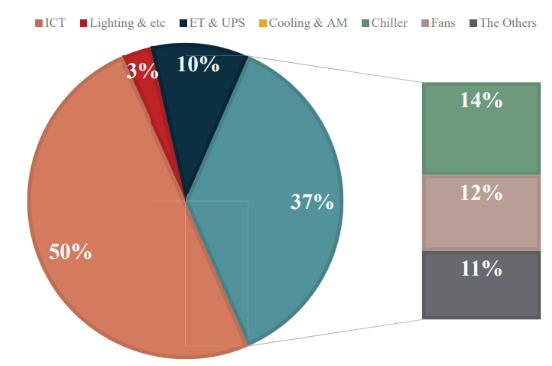
\includegraphics[scale=0.5]{../figures/consumo}
                    \caption{Consumo energético del CPD \cite{ZHANG2021102253}.}
                    \label{consumo_energetico}
                \end{center}
            \end{figure}        
        \end{column}
    \end{columns}    
\end{frame}

\begin{frame}{Green IT}
    Para reducir el impacto medioambiental de los CPDs se proponen diferentes soluciones, como pueden ser

    \begin{enumerate}
        \item Utilizar materiales de construcción sostenibles.
        \item Uso de energías renovables.
        \item Sistemas de refrigeración eficientes.
    \end{enumerate}
\end{frame}




\section{Sistemas de refrigeración de CPDs}

\subsection{Basados en aire}

\begin{frame}{Free Cooling}
    \begin{figure}
        \begin{center}
            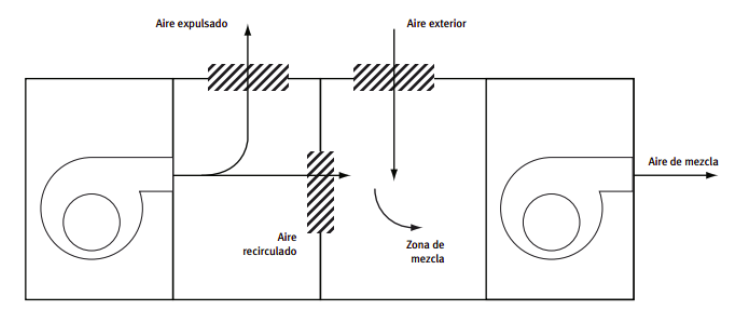
\includegraphics[scale=0.7]{../figures/free_cooling}
            \caption{Esquema del free cooling.}
            \label{free_coling}
        \end{center}
    \end{figure}
\end{frame}

\begin{frame}{Pasillos calientes y fríos}
    \begin{figure}
        \begin{center}
            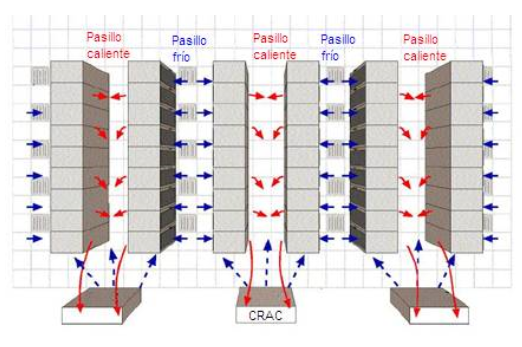
\includegraphics[scale=0.6]{../figures/pasillos}
            \caption{Esquema de los pasillos calientes y fríos. Fuente: \cite{Kelvion}.}
            \label{pasillos}
        \end{center}
    \end{figure}
\end{frame}

\begin{frame}{Confinamiento de zonas}
    \begin{figure}
        \begin{center}
            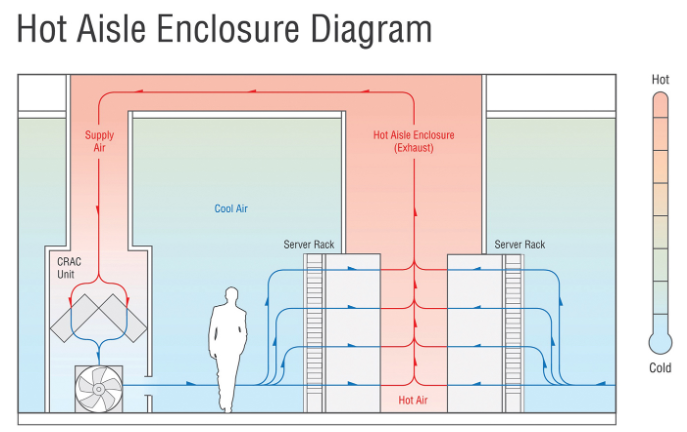
\includegraphics[scale=0.6]{../figures/hot_aisle}
            \caption{Diagrama de cerramiento de pasillo caliente. Fuente: \cite{journal-uptimeinstitute}.}
            \label{hot_aisle}
        \end{center}
    \end{figure}
\end{frame}

\begin{frame}{Refrigeración adiabática}
    \begin{itemize}
        \item Utiliza la baja humedad relativa del aire para incorporar agua y evaporarla.
    \end{itemize}
    \begin{figure}
        \begin{center}
            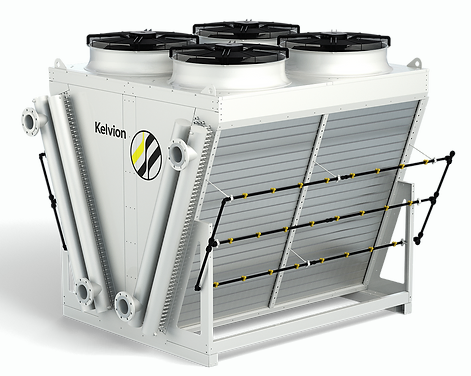
\includegraphics[scale=0.3]{../figures/adiabatic_coolers}
            \caption{Enfriamientos adiabáticos. Fuente: \cite{Kelvion}.}
            \label{adiabatic_coolers}
        \end{center}
    \end{figure}
\end{frame}

\begin{frame}{Falsos suelos y techos}
    \begin{itemize}
        \item Se instalan a distintas alturas $\rightarrow$ flexibilidad.
        \item Los suelos suelen ser rejillas de ventilación.
        \item Facilitan el acceso al cableado.
    \end{itemize}
\end{frame}

\begin{frame}{Otras técnicas}
    \begin{itemize}
        \item CRAC.
        \item CRAH.
        \item In-Rack Heat Extraction.
        \item Refrigeración vectorial calibrada (CVC).
        \item Expansión directa (DX cooling).
    \end{itemize}
\end{frame}



\subsection{Basados en agua}

\begin{frame}{Basados en agua}
    \begin{itemize}
        \item \textbf{Sistema de agua helada.} Enfría el aire con agua helada.
        \item \textbf{Enfriamiento evaporativo.}
            \begin{enumerate}
                \item Expone el aire caliente al agua.
                \item Se evapora el agua.
                \item Se extrae el calor del aire.
            \end{enumerate}
    \end{itemize}
\end{frame}



\subsection{Basados en inmersión}

\begin{frame}{Cómo funciona la inmersión}
    \begin{enumerate}
        \item El hardware se sumerge en un fluido.
        \item El fluido es dieléctrico, no conductor y no inflamable.
        \item El líquido absorbe el calor.
        \item El agua se evapora, se condensa y vuelve al líquido.
        \item El líquido se enfría.
    \end{enumerate}
\end{frame}

\section{Soluciones propietarias}

\begin{frame}{Empresas}
    \begin{columns}
        \begin{column}{0.5\textwidth}
            \begin{itemize}
                \item Especializadas en refrigeración por aire:
                \begin{itemize}
                    \item Usystems.
                    \item Munters.
                    \item Stulz.
                \end{itemize}

                \item Especializadas en refrigeración líquida:
                \begin{itemize}
                    \item LiquidStack
                    \item Submer
                    \item Green Revolution Cooling
                \end{itemize}
            \end{itemize}
        
            
        \end{column}
        \begin{column}{0.5\textwidth}
            \begin{figure}
                \begin{center}
                    
\includegraphics[scale=0.15]{./figures/usystems}
                    
\includegraphics[scale=0.2]{./figures/munters}

                \end{center}
            \end{figure}
        
            \begin{figure}
                \begin{center}
                    
\includegraphics[scale=0.2]{./figures/stulz}
                    
\includegraphics[scale=0.2]{./figures/liquidstack}
                \end{center}
            \end{figure}

            \begin{figure}
                \begin{center}
                    
\includegraphics[scale=0.2]{./figures/submer}
                    
\includegraphics[scale=0.2]{./figures/grc}

                \end{center}
            \end{figure}

        \end{column}
    \end{columns}

\end{frame}


\begin{frame}{Otras empresas}
    \begin{columns}
        \begin{column}{0.5\textwidth}
            \begin{itemize}
                \item Systemair
                \item Clysema
                \item Kelvion
            \end{itemize}
        
            \begin{figure}
                \begin{center}
                    
\includegraphics[scale=0.7]{./figures/systemair}
                \end{center}
            \end{figure}
        \end{column}

        \begin{column}{0.5\textwidth}      
            \begin{figure}
                \begin{center}
                    
\includegraphics[scale=0.35]{./figures/clysema}
                \end{center}
            \end{figure}
        
            \begin{figure}
                \begin{center}
                    
\includegraphics[scale=0.35]{./figures/kelvion}
                \end{center}
            \end{figure}
        \end{column}
    \end{columns}
\end{frame}




\section{Futuro}

\begin{frame}{Áreas de investigación}
    \begin{enumerate}
        \item Los CPDs han incrementado su potencia y número $\rightarrow$ Búsqueda de métodos de enfriamiento más eficaces y eficientes.
        \item Investigación enfocada principalmente en la refrigeración líquida.
    \end{enumerate}
\end{frame}

\begin{frame}{Técnicas en investigación}
    \begin{enumerate}
        \item Tecnologías de refrigeración líquida
        \item Refrigeración directa del chip
    \end{enumerate}
\end{frame}




\section{Conclusiones}

\begin{frame}{Conclusiones}
    \begin{enumerate}
        \item \textbf{Distintas vías de climatización:} Aire, agua e inmersión.
        \item La distribución de los componentes en el CPD tiene un impacto en la refrigeración.. 
        \item Las técnicas de refrigeración basadas en \textbf{refrigeración líquida} son las más \textbf{efectivas}.
        \item Evitar técnicas que requieran una cantidad excesiva de energía o produzcan contaminantes.
    \end{enumerate}
\end{frame}

\begin{frame}{Referencias}
    \bibliography{../bib/library.bib}
    \bibliographystyle{plain}
\end{frame}


\end{document}
